\documentclass[aspectratio=169]{beamer}
\geometry{paperwidth=320mm,paperheight=180mm}
\usepackage{fontspec}
\setmainfont[Path=fonts/,FontIndex=7,BoldFont=AvenirNext.ttc,BoldFeatures={FontIndex=2},ItalicFont=AvenirNext.ttc,ItalicFeatures={FontIndex=4},BoldItalicFont=AvenirNext.ttc,BoldItalicFeatures={FontIndex=3}]{AvenirNext.ttc}
\setsansfont[Path=fonts/,FontIndex=7,BoldFont=AvenirNext.ttc,BoldFeatures={FontIndex=2},ItalicFont=AvenirNext.ttc,ItalicFeatures={FontIndex=4},BoldItalicFont=AvenirNext.ttc,BoldItalicFeatures={FontIndex=3}]{AvenirNext.ttc}
\newfontfamily\heavy[Path=fonts/,FontIndex=2]{AvenirNext.ttc}
\setmonofont[Path=fonts/,BoldFont=JetBrainsMono-Bold.ttf,ItalicFont=JetBrainsMono-Italic.ttf,Contextuals=NoAlternate,Ligatures=NoCommon]{JetBrainsMono-Regular.ttf}
\usepackage{xcolor,graphicx,tikz,booktabs,tabularx,listings,amsmath}
\usetikzlibrary{arrows.meta,positioning}
\definecolor{paper}{HTML}{FFFFFF}
\definecolor{ink}{HTML}{252525}
\definecolor{teal}{HTML}{252525}
\definecolor{orange}{HTML}{777777}
\definecolor{wash}{HTML}{EAEAEA}
\definecolor{quiet}{HTML}{666666}
\definecolor{lightink}{HTML}{D0D0D0}
\definecolor{codepaper}{HTML}{F6F6F4}
\lstset{language=Python,basicstyle=\ttfamily\fontsize{9.5}{13}\selectfont\color{ink},keywordstyle=\bfseries\color{ink},commentstyle=\itshape\color{quiet},stringstyle=\color{ink},showstringspaces=false,columns=fullflexible,keepspaces=true,breaklines=true,breakatwhitespace=true,numbers=none,upquote=true,aboveskip=8pt,belowskip=6pt}
\hyphenpenalty=4000
\emergencystretch=3em
% The same two-line navigation and fine rule as the reference, without a candy motif.
\newcommand{\guideheader}[2]{\begin{tikzpicture}[remember picture,overlay]
\node[anchor=north west,inner sep=0,text width=176mm] at ([xshift=16mm,yshift=-7mm]current page.north west) {\fontsize{8.5}{10}\selectfont\color{quiet}#1};
\node[anchor=north west,inner sep=0,text width=176mm] at ([xshift=16mm,yshift=-11.5mm]current page.north west) {\heavy\fontsize{10}{12}\selectfont\color{ink}#2};
\draw[lightink,line width=.4pt] ([xshift=16mm,yshift=-17mm]current page.north west)--([xshift=192mm,yshift=-17mm]current page.north west);
\end{tikzpicture}}

\usepackage{colortbl}
\usetikzlibrary{fit}
\newsavebox{\codebox}
\setbeamercolor{normal text}{fg=ink,bg=paper}
\setbeamertemplate{navigation symbols}{}\setbeamertemplate{footline}{}\setbeamertemplate{headline}{}
\begin{document}
\begin{frame}[plain,fragile]\begin{tikzpicture}[remember picture,overlay,x=1cm,y=1cm]\begin{scope}[shift={(current page.south west)}]
\node[anchor=north west,inner sep=0pt,text width=29cm,align=left,text=teal,font=\fontsize{16}{\dimexpr16pt*6/5\relax}\selectfont] at (1.5,16.5) {\heavy LESSON 4};
\node[anchor=north west,inner sep=0pt,text width=29cm,align=left,text=ink,font=\fontsize{46}{\dimexpr46pt*6/5\relax}\selectfont] at (1.5,14.4) {\heavy Fruit\\Feast};
\node[anchor=north west,inner sep=0pt,text width=29cm,align=left,text=quiet,font=\fontsize{22}{\dimexpr22pt*6/5\relax}\selectfont] at (1.5,9.3) {Track what is possible};
\node[anchor=south,inner sep=0] at (16,2.3) {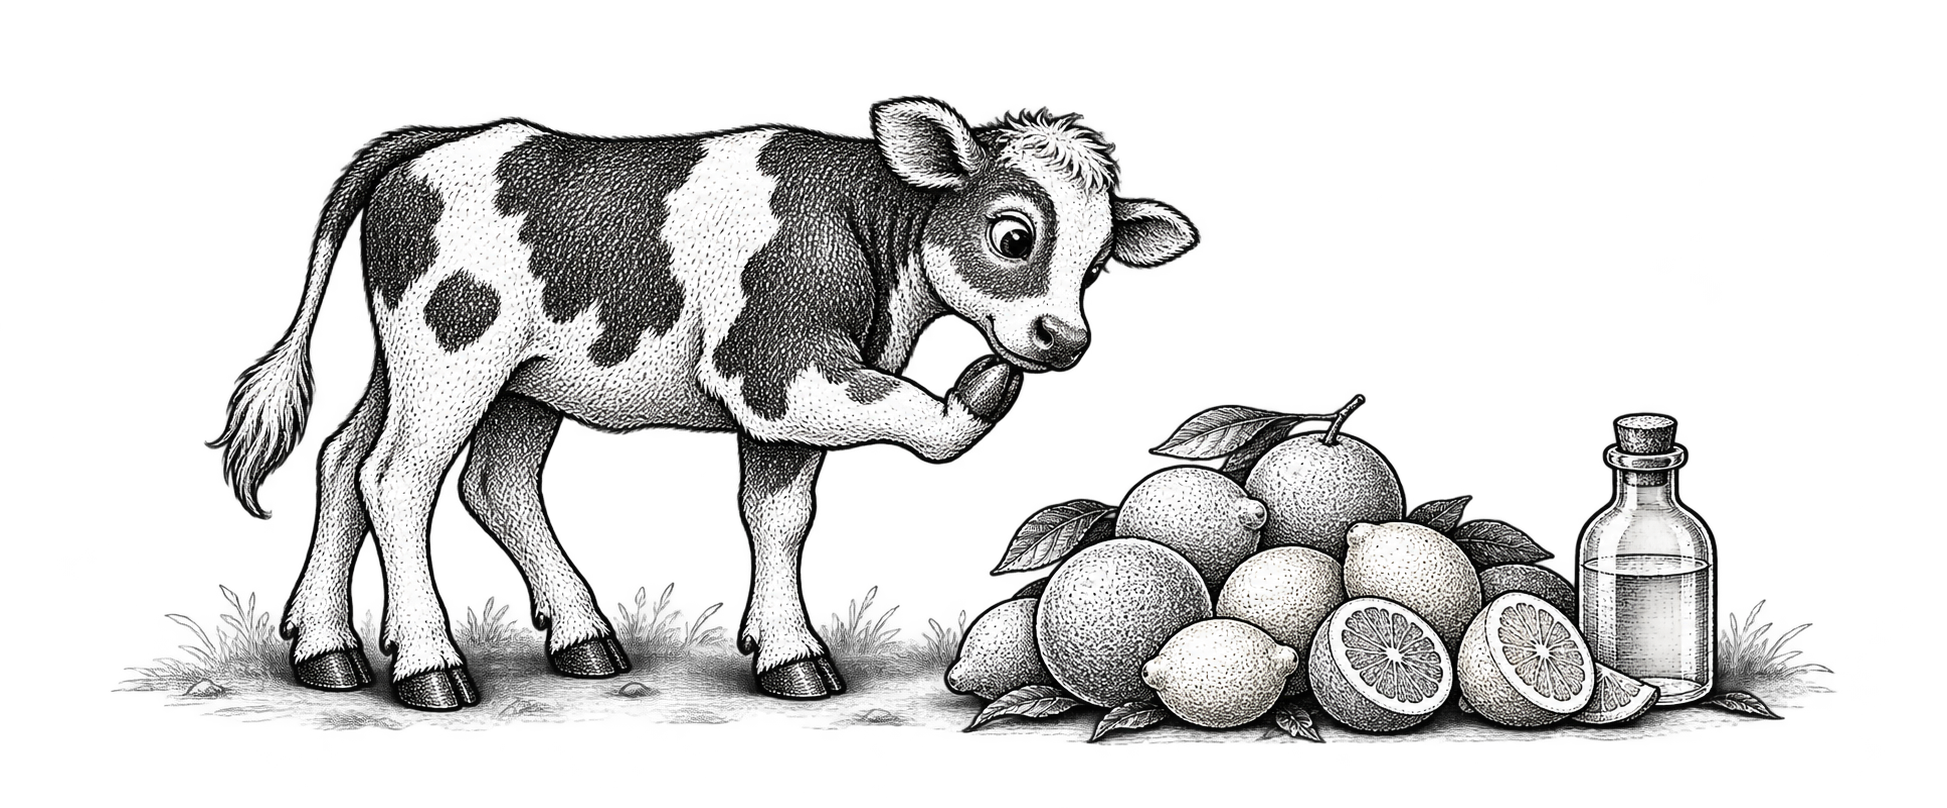
\includegraphics[width=27cm,height=6cm,keepaspectratio]{assets/cover.png}};\node[anchor=west,inner sep=0] at (1.5,1) {
\includegraphics[width=3.8cm]{assets/logo.png}};\node[anchor=east,inner sep=0] at (30.5,1) {
\includegraphics[width=5.5cm]{assets/julians-pathfinder-monochrome.pdf}};
\node[anchor=north west,inner sep=0pt,text width=1cm,align=left,text=quiet,font=\fontsize{11}{\dimexpr11pt*6/5\relax}\selectfont] at (15.8,0.8) {\insertframenumber};
\node[anchor=north west,inner sep=0pt,text width=12cm,align=left,text=ink,font=\fontsize{14}{\dimexpr14pt*6/5\relax}\selectfont] at (18,16.5) {\href{https://colab.research.google.com/github/fifteen02/julians-pathfinder/blob/main/Lesson\%204/lesson.ipynb}{\underline{Open this lesson in Google Colab}}};
\end{scope}\end{tikzpicture}
\end{frame}

\begin{frame}[plain,fragile]\begin{tikzpicture}[remember picture,overlay,x=1cm,y=1cm]\begin{scope}[shift={(current page.south west)}]
\node[anchor=north west,inner sep=0pt,text width=29cm,align=left,text=quiet,font=\fontsize{13}{\dimexpr13pt*6/5\relax}\selectfont] at (1.5,16.9) {\heavy LESSON 4 / TODAY};
\node[anchor=north west,inner sep=0pt,text width=1cm,align=left,text=quiet,font=\fontsize{11}{\dimexpr11pt*6/5\relax}\selectfont] at (30,0.8) {\insertframenumber};
\node[anchor=north west,inner sep=0pt,text width=29cm,align=left,text=quiet,font=\fontsize{18}{\dimexpr18pt*6/5\relax}\selectfont] at (1.5,15.4) {\heavy MAIN IDEA};
\node[anchor=north west,inner sep=0pt,text width=29cm,align=left,text=ink,font=\fontsize{40}{\dimexpr40pt*6/5\relax}\selectfont] at (1.5,14.3) {\heavy Track what is possible.};
\node(idea)[anchor=north west,inner sep=0pt,text width=28cm,align=left,text=ink,font=\fontsize{24}{\dimexpr24pt*6/5\relax}\selectfont] at (1.5,11.9) {Store yes or no for every fullness you can reach, and remember whether the water has been used.};
\node[anchor=north west,inner sep=0pt,text width=28cm,align=left,font=\fontsize{24}{30}\selectfont] at ([yshift=-9mm]idea.south west) {\textbf{You will be able to}\par\smallskip\hangindent=1.1em\hangafter=1\textbullet\ mark which fullness values can be reached, without counting routes;\par\hangindent=1.1em\hangafter=1\textbullet\ explain why we must remember whether the water has been used;\par\hangindent=1.1em\hangafter=1\textbullet\ find the values before water, just after drinking, and after more fruit.\par};
\end{scope}\end{tikzpicture}
\end{frame}

\begin{frame}[plain,fragile]\begin{tikzpicture}[remember picture,overlay,x=1cm,y=1cm]\begin{scope}[shift={(current page.south west)}]
\node[anchor=north west,inner sep=0pt,text width=29cm,align=left,text=quiet,font=\fontsize{13}{\dimexpr13pt*6/5\relax}\selectfont] at (1.5,16.9) {\heavy LESSON 4 / L4-01 / QUESTION};
\node[anchor=north west,inner sep=0pt,text width=1cm,align=left,text=quiet,font=\fontsize{11}{\dimexpr11pt*6/5\relax}\selectfont] at (30,0.8) {\insertframenumber};
\node[anchor=north west,inner sep=0pt,text width=29cm,align=left,text=ink,font=\fontsize{34}{\dimexpr34pt*6/5\relax}\selectfont] at (1.5,15.4) {\heavy Eating without going over};
\node(body)[anchor=north west,inner sep=0pt,text width=29cm,align=left,text=ink,font=\fontsize{25}{\dimexpr25pt*6/5\relax}\selectfont] at (1.5,12.4) {Fullness starts at 0 and must never exceed 10. An orange adds 4 and a lemon adds 7. You may eat either fruit repeatedly. Without water, what fullness values are reachable?};
\node[anchor=south,inner sep=0] at (16,2.1) {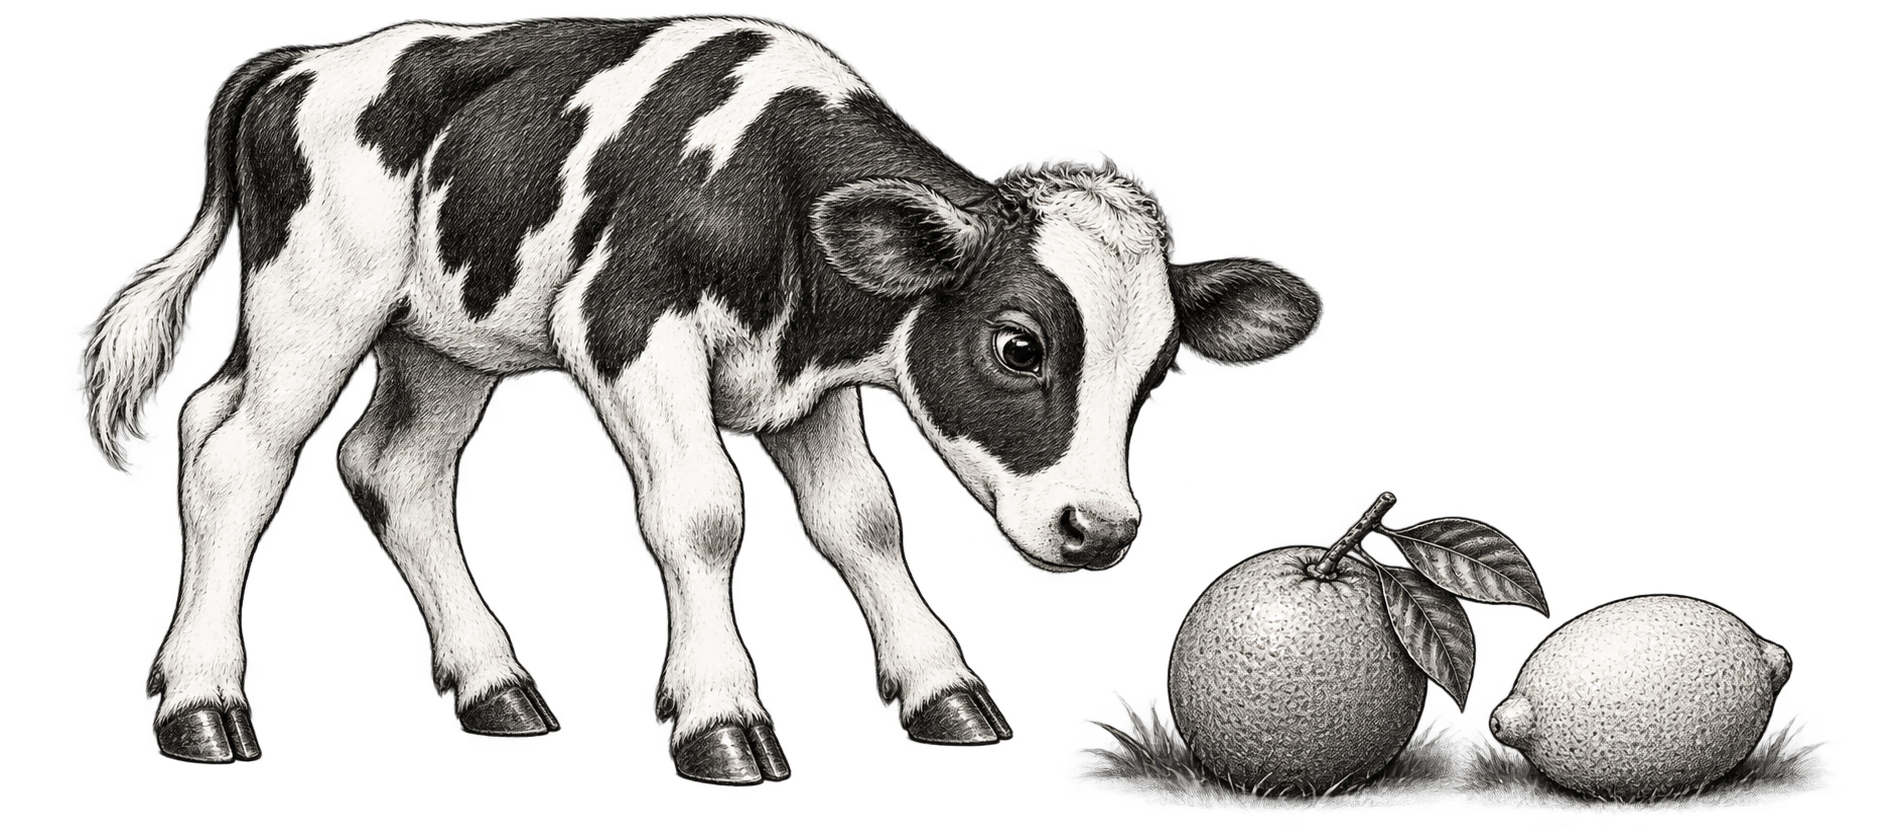
\includegraphics[width=21cm,height=6.0cm,keepaspectratio]{assets/slides/fruit.png}};
\node[anchor=north west,inner sep=0pt,text width=28cm,align=left,text=quiet,font=\fontsize{17}{\dimexpr17pt*6/5\relax}\selectfont] at (1.5,1.45) {Think on your own first. Then compare your reasoning with a partner.};
\end{scope}\end{tikzpicture}
\end{frame}

\begin{frame}[plain,fragile]\begin{tikzpicture}[remember picture,overlay,x=1cm,y=1cm]\begin{scope}[shift={(current page.south west)}]
\node[anchor=north west,inner sep=0pt,text width=29cm,align=left,text=quiet,font=\fontsize{13}{\dimexpr13pt*6/5\relax}\selectfont] at (1.5,16.9) {\heavy LESSON 4 / L4-01 / ANSWER};
\node[anchor=north west,inner sep=0pt,text width=1cm,align=left,text=quiet,font=\fontsize{11}{\dimexpr11pt*6/5\relax}\selectfont] at (30,0.8) {\insertframenumber};
\node[anchor=north west,inner sep=0pt,text width=29cm,align=left,text=ink,font=\fontsize{34}{\dimexpr34pt*6/5\relax}\selectfont] at (1.5,15.4) {\heavy Eating without going over};
\node(body)[anchor=north west,inner sep=0pt,text width=29cm,align=left,text=ink,font=\fontsize{25}{\dimexpr25pt*6/5\relax}\selectfont] at (1.5,12.4) {The reachable values are 0, 4, 7 and 8. The best is 8. Eating 4 then 7 would reach 11, so that action is forbidden rather than clipped back to 10.};
\node[anchor=north west,inner sep=0pt,text width=28cm,align=left,text=teal,font=\fontsize{21}{\dimexpr21pt*6/5\relax}\selectfont] at (1.5,4.0) {\textbf{Watch for:} Reachable values need not form a continuous interval.};
\end{scope}\end{tikzpicture}
\end{frame}

\begin{frame}[plain,fragile]\begin{tikzpicture}[remember picture,overlay,x=1cm,y=1cm]\begin{scope}[shift={(current page.south west)}]
\node[anchor=north west,inner sep=0pt,text width=29cm,align=left,text=quiet,font=\fontsize{13}{\dimexpr13pt*6/5\relax}\selectfont] at (1.5,16.9) {\heavy LESSON 4 / L4-02 / QUESTION};
\node[anchor=north west,inner sep=0pt,text width=1cm,align=left,text=quiet,font=\fontsize{11}{\dimexpr11pt*6/5\relax}\selectfont] at (30,0.8) {\insertframenumber};
\node[anchor=north west,inner sep=0pt,text width=29cm,align=left,text=ink,font=\fontsize{34}{\dimexpr34pt*6/5\relax}\selectfont] at (1.5,15.4) {\heavy Water can make room};
\node(body)[anchor=north west,inner sep=0pt,text width=29cm,align=left,text=ink,font=\fontsize{25}{\dimexpr25pt*6/5\relax}\selectfont] at (1.5,12.4) {At most once, the cow may drink water. Water halves the current fullness, rounding down. With limit 10 and fruit sizes 4 and 7, find a route to fullness 10.};
\node[anchor=south,inner sep=0] at (16,2.1) {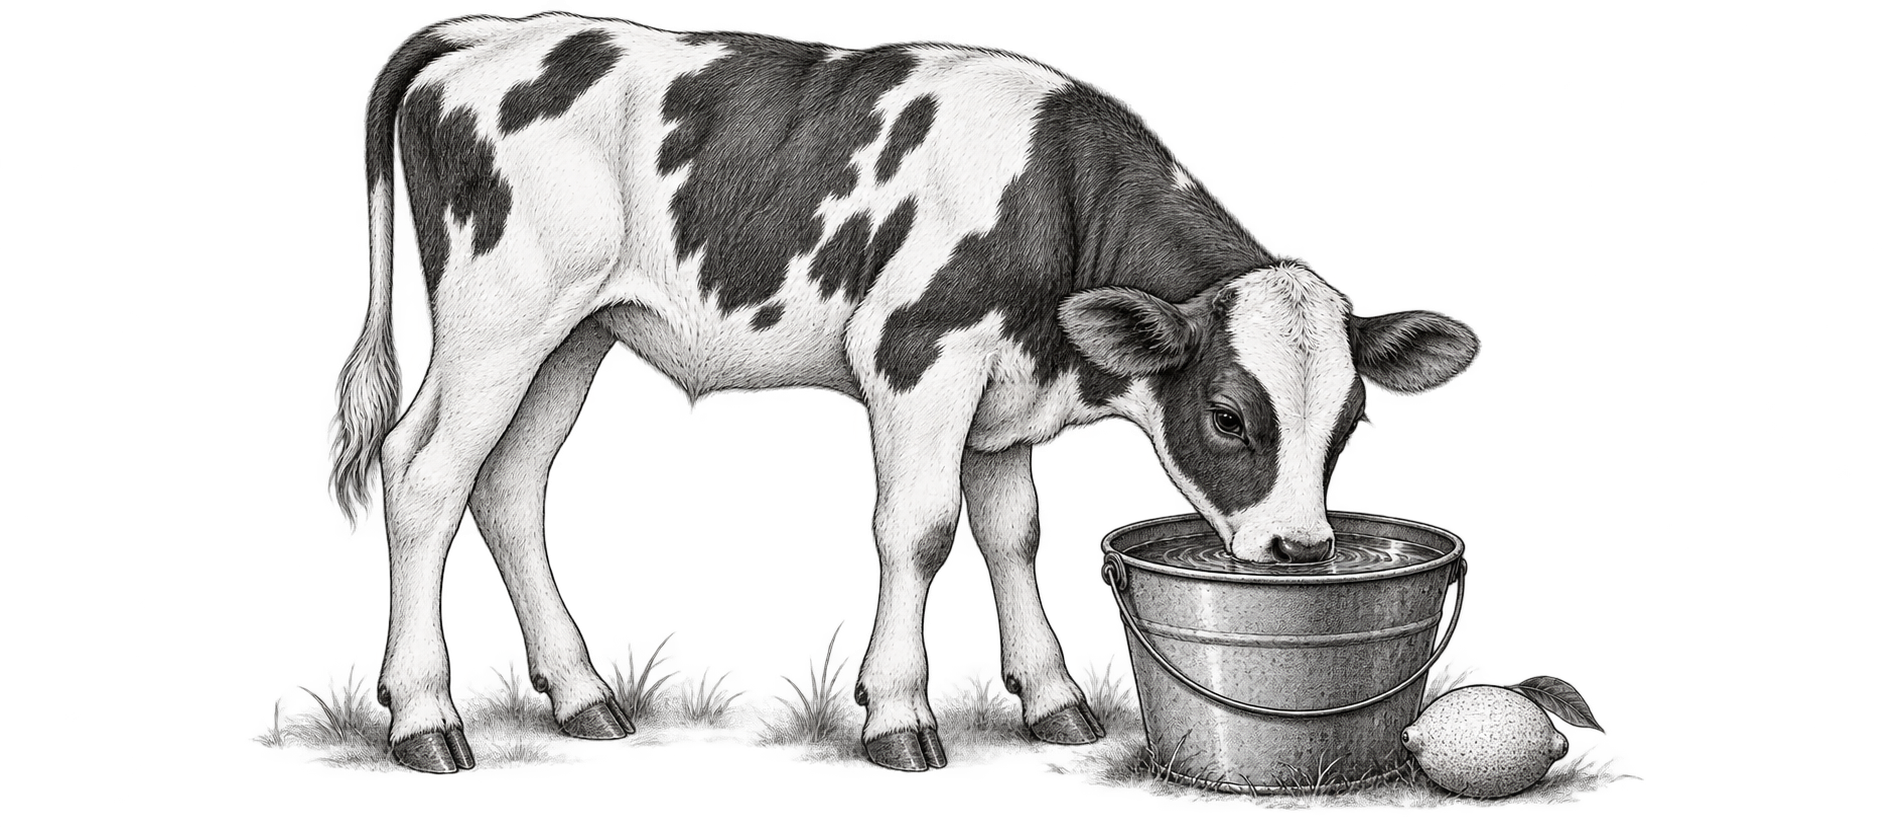
\includegraphics[width=21cm,height=6.0cm,keepaspectratio]{assets/slides/water.png}};
\node[anchor=north west,inner sep=0pt,text width=28cm,align=left,text=quiet,font=\fontsize{17}{\dimexpr17pt*6/5\relax}\selectfont] at (1.5,1.45) {Think on your own first. Then compare your reasoning with a partner.};
\end{scope}\end{tikzpicture}
\end{frame}

\begin{frame}[plain,fragile]\begin{tikzpicture}[remember picture,overlay,x=1cm,y=1cm]\begin{scope}[shift={(current page.south west)}]
\node[anchor=north west,inner sep=0pt,text width=29cm,align=left,text=quiet,font=\fontsize{13}{\dimexpr13pt*6/5\relax}\selectfont] at (1.5,16.9) {\heavy LESSON 4 / L4-02 / ANSWER};
\node[anchor=north west,inner sep=0pt,text width=1cm,align=left,text=quiet,font=\fontsize{11}{\dimexpr11pt*6/5\relax}\selectfont] at (30,0.8) {\insertframenumber};
\node[anchor=north west,inner sep=0pt,text width=29cm,align=left,text=ink,font=\fontsize{34}{\dimexpr34pt*6/5\relax}\selectfont] at (1.5,15.4) {\heavy Water can make room};
\node(body)[anchor=north west,inner sep=0pt,text width=29cm,align=left,text=ink,font=\fontsize{22}{\dimexpr22pt*6/5\relax}\selectfont] at (1.5,12.4) {Eat a lemon: 0 to 7. Drink: 7 // 2 = 3. Eat another lemon: 3 to 10. This reaches the limit exactly, so no better answer is possible.};
\node[anchor=north west,inner sep=0,text width=28cm] at (1.5,6.5) {\resizebox{18cm}{!}{\begin{minipage}{14cm}\begin{center}\begin{tikzpicture}[>=Stealth,every node/.style={font=\fontsize{13}{15}\selectfont},box/.style={draw=teal,rounded corners,minimum width=20mm,minimum height=8mm,fill=wash},arr/.style={->,thick,teal}]\node[box] (p0) at (0.0,0) {0};\node[box] (p1) at (3.6,0) {7};\node[box] (p2) at (7.2,0) {3};\node[box] (p3) at (10.8,0) {10};\draw[arr] (p0)--node[above=6mm]{eat 7}(p1);\draw[arr] (p1)--node[above=6mm]{water: // 2}(p2);\draw[arr] (p2)--node[above=6mm]{eat 7}(p3);\end{tikzpicture}\end{center}\end{minipage}}};
\end{scope}\end{tikzpicture}
\end{frame}

\begin{frame}[plain,fragile]\begin{tikzpicture}[remember picture,overlay,x=1cm,y=1cm]\begin{scope}[shift={(current page.south west)}]
\node[anchor=north west,inner sep=0pt,text width=29cm,align=left,text=quiet,font=\fontsize{13}{\dimexpr13pt*6/5\relax}\selectfont] at (1.5,16.9) {\heavy LESSON 4 / L4-03 / QUESTION};
\node[anchor=north west,inner sep=0pt,text width=1cm,align=left,text=quiet,font=\fontsize{11}{\dimexpr11pt*6/5\relax}\selectfont] at (30,0.8) {\insertframenumber};
\node[anchor=north west,inner sep=0pt,text width=29cm,align=left,text=ink,font=\fontsize{34}{\dimexpr34pt*6/5\relax}\selectfont] at (1.5,15.4) {\heavy Same fullness, different choices};
\node(body)[anchor=north west,inner sep=0pt,text width=29cm,align=left,text=ink,font=\fontsize{25}{\dimexpr25pt*6/5\relax}\selectfont] at (1.5,12.4) {A reachability flag is a yes/no answer: can the cow reach this situation? Compare fullness 4 with water still unused and fullness 4 after drinking. Do they allow the same next actions? Why would one flag called reachable[4] lose information we need?};
\node[anchor=north west,inner sep=0pt,text width=28cm,align=left,text=teal,font=\fontsize{22}{\dimexpr22pt*6/5\relax}\selectfont] at (1.5,4.0) {Think on your own first. Then compare your reasoning with a partner.};
\end{scope}\end{tikzpicture}
\end{frame}

\begin{frame}[plain,fragile]
\begin{tikzpicture}[remember picture,overlay,x=1cm,y=1cm]\begin{scope}[shift={(current page.south west)}]
\node[anchor=north west,inner sep=0pt,text width=29cm,align=left,text=quiet,font=\fontsize{13}{\dimexpr13pt*6/5\relax}\selectfont] at (1.5,16.9) {\heavy LESSON 4 / L4-03 / ANSWER};
\node[anchor=north west,inner sep=0pt,text width=1cm,align=left,text=quiet,font=\fontsize{11}{\dimexpr11pt*6/5\relax}\selectfont] at (30,0.8) {\insertframenumber};
\node[anchor=north west,inner sep=0pt,text width=29cm,align=left,text=ink,font=\fontsize{34}{\dimexpr34pt*6/5\relax}\selectfont] at (1.5,15.4) {\heavy Same fullness, different choices};
\node(body)[anchor=north west,inner sep=0pt,text width=29cm,align=left,text=ink,font=\fontsize{25}{\dimexpr25pt*6/5\relax}\selectfont] at (1.5,12.4) {No. Before water, drinking is still available. After water, it is forbidden. Use dry[4] for reachable without drinking and wet[4] for reachable after drinking.};
\node[anchor=north west,inner sep=0pt,text width=28cm,align=left,text=teal,font=\fontsize{21}{\dimexpr21pt*6/5\relax}\selectfont] at (1.5,4.0) {\textbf{Watch for:} Adding counts here answers how many routes there are, which the problem never asks.};
\end{scope}\end{tikzpicture}
\end{frame}

\begin{frame}[plain,fragile]\begin{tikzpicture}[remember picture,overlay,x=1cm,y=1cm]\begin{scope}[shift={(current page.south west)}]
\node[anchor=north west,inner sep=0pt,text width=29cm,align=left,text=quiet,font=\fontsize{13}{\dimexpr13pt*6/5\relax}\selectfont] at (1.5,16.9) {\heavy LESSON 4 / L4-04 / QUESTION};
\node[anchor=north west,inner sep=0pt,text width=1cm,align=left,text=quiet,font=\fontsize{11}{\dimexpr11pt*6/5\relax}\selectfont] at (30,0.8) {\insertframenumber};
\node[anchor=north west,inner sep=0pt,text width=29cm,align=left,text=ink,font=\fontsize{34}{\dimexpr34pt*6/5\relax}\selectfont] at (1.5,15.4) {\heavy A small recursive search};
\node(body)[anchor=north west,inner sep=0pt,text width=29cm,align=left,text=ink,font=\fontsize{20}{\dimexpr20pt*6/5\relax}\selectfont] at (1.5,12.4) {Write feast\_cached(limit, a, b) using cached recursion. The helper asks: from fullness f, with used\_water saying whether the drink has been used, what is the greatest final fullness reachable? List every legal next action, including stopping. Explain why f and used\_water belong in the cache key.};
\node(sig)[anchor=north west,inner sep=3mm,fill=codepaper,align=left,font=\ttfamily\fontsize{16}{20}\selectfont] at ([yshift=-4mm,xshift=3mm]body.south west) {def feast\_cached(limit, a, b):\\\hspace*{2.4em}def best(fullness, used\_water):\\\hspace*{4.8em}return None  \# Replace this\\\hspace*{2.4em}return best(0, False)};
\node(result)[anchor=north west,inner sep=0pt,text width=13.5cm,align=left,text=quiet,font=\fontsize{17}{20}\selectfont] at ([yshift=-4mm,xshift=15.5cm]body.south west) {\textbf{Returns}\par \textbf{feast\_cached(limit, a, b)}: the greatest reachable fullness, starting empty with water unused.\par\smallskip \textbf{best(fullness, used\_water)}: the greatest final fullness reachable from this fullness and water status.\par\smallskip };
\node(both)[fit=(sig)(result),inner sep=0] {};
\node[anchor=north west,inner sep=0pt,text width=29cm,align=left,text=quiet,font=\fontsize{18}{22}\selectfont] at ([yshift=-3mm,xshift=-3mm]both.south west) {\textbf{Hints.} Stopping is always allowed. What does that give as a first answer? Which moves are legal from (fullness, used\_water)? Which move changes used\_water, and can it happen twice?};
\end{scope}\end{tikzpicture}
\end{frame}

\begin{frame}[plain,fragile]\begin{tikzpicture}[remember picture,overlay,x=1cm,y=1cm]\begin{scope}[shift={(current page.south west)}]
\node[anchor=north west,inner sep=0pt,text width=29cm,align=left,text=quiet,font=\fontsize{13}{\dimexpr13pt*6/5\relax}\selectfont] at (1.5,16.9) {\heavy LESSON 4 / L4-04 / ANSWER};
\node[anchor=north west,inner sep=0pt,text width=1cm,align=left,text=quiet,font=\fontsize{11}{\dimexpr11pt*6/5\relax}\selectfont] at (30,0.8) {\insertframenumber};
\node[anchor=north west,inner sep=0pt,text width=29cm,align=left,text=ink,font=\fontsize{34}{\dimexpr34pt*6/5\relax}\selectfont] at (1.5,15.4) {\heavy A small recursive search};
\node(body)[anchor=north west,inner sep=0pt,text width=29cm,align=left,text=ink,font=\fontsize{25}{\dimexpr25pt*6/5\relax}\selectfont] at (1.5,12.4) {Try either fruit if it fits, and water only if it is unused. Also allow stopping at the current fullness. Cache the best final fullness for each pair. The same fullness with a different water status has different legal futures.};
\node[anchor=north west,inner sep=0pt,text width=28cm,align=left,text=teal,font=\fontsize{21}{\dimexpr21pt*6/5\relax}\selectfont] at (1.5,4.0) {\textbf{Watch for:} Recursing from wet to dry would incorrectly make another drink available.};
\end{scope}\end{tikzpicture}
\end{frame}

\begin{frame}[plain,fragile]
\begin{lrbox}{\codebox}\begin{minipage}{790pt}
\begin{lstlisting}[basicstyle=\ttfamily\fontsize{17.5}{19.6}\selectfont\color{ink},numbers=left,numberstyle=\ttfamily\fontsize{11.4}{19.6}\selectfont\color{quiet},numbersep=12pt,xleftmargin=28pt,firstnumber=1,breaklines=false,aboveskip=0pt,belowskip=0pt]
from functools import lru_cache

def feast_cached(limit, a, b):
    @lru_cache(None)
    def best(fullness, used_water):
        answer = fullness
        for fruit in (a, b):
            if fullness + fruit <= limit:
                answer = max(answer, best(fullness + fruit, used_water))
        if not used_water:
            answer = max(answer, best(fullness // 2, True))
        return answer
    return best(0, False)
\end{lstlisting}
\end{minipage}\end{lrbox}
\begin{tikzpicture}[remember picture,overlay,x=1cm,y=1cm]\begin{scope}[shift={(current page.south west)}]
\node[anchor=north west,inner sep=0pt,text width=29cm,align=left,text=quiet,font=\fontsize{13}{\dimexpr13pt*6/5\relax}\selectfont] at (1.5,16.9) {\heavy LESSON 4 / L4-04 / ANSWER: PYTHON};
\node[anchor=north west,inner sep=0pt,text width=1cm,align=left,text=quiet,font=\fontsize{11}{\dimexpr11pt*6/5\relax}\selectfont] at (30,0.8) {\insertframenumber};
\node[anchor=north west,inner sep=0pt,text width=29cm,align=left,text=ink,font=\fontsize{34}{40.8}\selectfont] at (1.5,15.4) {\heavy feast cached};
\node[anchor=north,inner sep=5mm,fill=codepaper] at (16,13.6) {\usebox{\codebox}};
\end{scope}\end{tikzpicture}

\end{frame}

\begin{frame}[plain,fragile]\begin{tikzpicture}[remember picture,overlay,x=1cm,y=1cm]\begin{scope}[shift={(current page.south west)}]
\node[anchor=north west,inner sep=0pt,text width=29cm,align=left,text=quiet,font=\fontsize{13}{\dimexpr13pt*6/5\relax}\selectfont] at (1.5,16.9) {\heavy LESSON 4 / L4-05 / QUESTION};
\node[anchor=north west,inner sep=0pt,text width=1cm,align=left,text=quiet,font=\fontsize{11}{\dimexpr11pt*6/5\relax}\selectfont] at (30,0.8) {\insertframenumber};
\node[anchor=north west,inner sep=0pt,text width=29cm,align=left,text=ink,font=\fontsize{34}{\dimexpr34pt*6/5\relax}\selectfont] at (1.5,15.4) {\heavy First, all fullness values before water};
\node(body)[anchor=north west,inner sep=0pt,text width=29cm,align=left,text=ink,font=\fontsize{22}{\dimexpr22pt*6/5\relax}\selectfont] at (1.5,12.4) {For limit 10 and fruit sizes 4 and 7, fill dry[0] through dry[10]. Why can the scan run from low fullness to high fullness?};
\node(tab)[anchor=north west,inner sep=0,text width=29cm] at ([yshift=-8mm]body.south west) {\begingroup\fontsize{22}{26}\selectfont\setlength{\tabcolsep}{5pt}\setlength{\arrayrulewidth}{.5pt}\arrayrulecolor{quiet}\renewcommand{\arraystretch}{1}\begin{tabularx}{\linewidth}{|>{\raggedright\arraybackslash}p{52mm}|>{\centering\arraybackslash}X|>{\centering\arraybackslash}X|>{\centering\arraybackslash}X|>{\centering\arraybackslash}X|>{\centering\arraybackslash}X|>{\centering\arraybackslash}X|>{\centering\arraybackslash}X|>{\centering\arraybackslash}X|>{\centering\arraybackslash}X|>{\centering\arraybackslash}X|>{\centering\arraybackslash}X|}\hline
\rowcolor{wash}\rule[-3mm]{0pt}{9.5mm}\textbf{Fullness f} & \textbf{0} & \textbf{1} & \textbf{2} & \textbf{3} & \textbf{4} & \textbf{5} & \textbf{6} & \textbf{7} & \textbf{8} & \textbf{9} & \textbf{10}\\\hline
\rule[-4.6mm]{0pt}{13.5mm}dry[f] & Y &  &  &  &  &  &  &  &  &  & \\\hline
\end{tabularx}\endgroup};
\end{scope}\end{tikzpicture}
\end{frame}

\begin{frame}[plain,fragile]\begin{tikzpicture}[remember picture,overlay,x=1cm,y=1cm]\begin{scope}[shift={(current page.south west)}]
\node[anchor=north west,inner sep=0pt,text width=29cm,align=left,text=quiet,font=\fontsize{13}{\dimexpr13pt*6/5\relax}\selectfont] at (1.5,16.9) {\heavy LESSON 4 / L4-05 / ANSWER};
\node[anchor=north west,inner sep=0pt,text width=1cm,align=left,text=quiet,font=\fontsize{11}{\dimexpr11pt*6/5\relax}\selectfont] at (30,0.8) {\insertframenumber};
\node[anchor=north west,inner sep=0pt,text width=29cm,align=left,text=ink,font=\fontsize{34}{\dimexpr34pt*6/5\relax}\selectfont] at (1.5,15.4) {\heavy First, all fullness values before water};
\node(body)[anchor=north west,inner sep=0pt,text width=29cm,align=left,text=ink,font=\fontsize{22}{\dimexpr22pt*6/5\relax}\selectfont] at (1.5,12.4) {Only dry[0], dry[4], dry[7] and dry[8] are true. Fruit adds a positive amount, so it always moves to a larger index. A forward scan reaches those new states later.};
\node(tab)[anchor=north west,inner sep=0,text width=29cm] at ([yshift=-8mm]body.south west) {\begingroup\fontsize{22}{26}\selectfont\setlength{\tabcolsep}{5pt}\setlength{\arrayrulewidth}{.5pt}\arrayrulecolor{quiet}\renewcommand{\arraystretch}{1}\begin{tabularx}{\linewidth}{|>{\raggedright\arraybackslash}p{52mm}|>{\centering\arraybackslash}X|>{\centering\arraybackslash}X|>{\centering\arraybackslash}X|>{\centering\arraybackslash}X|>{\centering\arraybackslash}X|>{\centering\arraybackslash}X|>{\centering\arraybackslash}X|>{\centering\arraybackslash}X|>{\centering\arraybackslash}X|>{\centering\arraybackslash}X|>{\centering\arraybackslash}X|}\hline
\rowcolor{wash}\rule[-3mm]{0pt}{9.5mm}\textbf{Fullness f} & \textbf{0} & \textbf{1} & \textbf{2} & \textbf{3} & \textbf{4} & \textbf{5} & \textbf{6} & \textbf{7} & \textbf{8} & \textbf{9} & \textbf{10}\\\hline
\rule[-4.6mm]{0pt}{13.5mm}dry[f] & Y & - & - & - & Y & - & - & Y & Y & - & -\\\hline
\end{tabularx}\endgroup};
\end{scope}\end{tikzpicture}
\end{frame}

\begin{frame}[plain,fragile]\begin{tikzpicture}[remember picture,overlay,x=1cm,y=1cm]\begin{scope}[shift={(current page.south west)}]
\node[anchor=north west,inner sep=0pt,text width=29cm,align=left,text=quiet,font=\fontsize{13}{\dimexpr13pt*6/5\relax}\selectfont] at (1.5,16.9) {\heavy LESSON 4 / L4-06 / QUESTION};
\node[anchor=north west,inner sep=0pt,text width=1cm,align=left,text=quiet,font=\fontsize{11}{\dimexpr11pt*6/5\relax}\selectfont] at (30,0.8) {\insertframenumber};
\node[anchor=north west,inner sep=0pt,text width=29cm,align=left,text=ink,font=\fontsize{34}{\dimexpr34pt*6/5\relax}\selectfont] at (1.5,15.4) {\heavy Then, drink from every dry state};
\node(body)[anchor=north west,inner sep=0pt,text width=29cm,align=left,text=ink,font=\fontsize{25}{\dimexpr25pt*6/5\relax}\selectfont] at (1.5,12.4) {Take every fullness you marked as reachable without water in L4-05. Halve each one, rounding down, to find the states immediately after drinking and before any further fruit. Why would drinking only from the largest dry value miss a useful possibility?};
\node[anchor=north west,inner sep=0pt,text width=28cm,align=left,text=teal,font=\fontsize{22}{\dimexpr22pt*6/5\relax}\selectfont] at (1.5,4.0) {Think on your own first. Then compare your reasoning with a partner.};
\end{scope}\end{tikzpicture}
\end{frame}

\begin{frame}[plain,fragile]\begin{tikzpicture}[remember picture,overlay,x=1cm,y=1cm]\begin{scope}[shift={(current page.south west)}]
\node[anchor=north west,inner sep=0pt,text width=29cm,align=left,text=quiet,font=\fontsize{13}{\dimexpr13pt*6/5\relax}\selectfont] at (1.5,16.9) {\heavy LESSON 4 / L4-06 / ANSWER};
\node[anchor=north west,inner sep=0pt,text width=1cm,align=left,text=quiet,font=\fontsize{11}{\dimexpr11pt*6/5\relax}\selectfont] at (30,0.8) {\insertframenumber};
\node[anchor=north west,inner sep=0pt,text width=29cm,align=left,text=ink,font=\fontsize{34}{\dimexpr34pt*6/5\relax}\selectfont] at (1.5,15.4) {\heavy Then, drink from every dry state};
\node(body)[anchor=north west,inner sep=0pt,text width=29cm,align=left,text=ink,font=\fontsize{22}{\dimexpr22pt*6/5\relax}\selectfont] at (1.5,12.4) {The immediate-after-water values are 0, 2, 3 and 4: halve 0, 4, 7 and 8 respectively. Drinking at fullness 7 gives 3, then eating a fruit of size 7 reaches 10. Drinking only at fullness 8 gives 4, from which the largest reachable value is 8. It misses the best route.};
\node[anchor=north west,inner sep=0,text width=28cm] at (1.5,6.5) {\resizebox{18cm}{!}{\begin{minipage}{14cm}\begin{center}\begin{tikzpicture}[>=Stealth,every node/.style={font=\fontsize{13}{15}\selectfont},box/.style={draw=teal,rounded corners,minimum width=20mm,minimum height=8mm,fill=wash},arr/.style={->,thick,teal}]\node[anchor=east] at (-1,0) {dry};\node[anchor=east] at (-1,-2) {just drank};\node[box] (a0) at (0.0,0) {0};\node[box] (b0) at (0.0,-2) {0};\draw[arr,orange] (a0)--node[right]{// 2}(b0);\node[box] (a1) at (2.8,0) {4};\node[box] (b1) at (2.8,-2) {2};\draw[arr,orange] (a1)--node[right]{// 2}(b1);\node[box] (a2) at (5.6,0) {7};\node[box] (b2) at (5.6,-2) {3};\draw[arr,orange] (a2)--node[right]{// 2}(b2);\node[box] (a3) at (8.399999999999999,0) {8};\node[box] (b3) at (8.399999999999999,-2) {4};\draw[arr,orange] (a3)--node[right]{// 2}(b3);\end{tikzpicture}\end{center}\end{minipage}}};
\end{scope}\end{tikzpicture}
\end{frame}

\begin{frame}[plain,fragile]\begin{tikzpicture}[remember picture,overlay,x=1cm,y=1cm]\begin{scope}[shift={(current page.south west)}]
\node[anchor=north west,inner sep=0pt,text width=29cm,align=left,text=quiet,font=\fontsize{13}{\dimexpr13pt*6/5\relax}\selectfont] at (1.5,16.9) {\heavy LESSON 4 / L4-07 / QUESTION};
\node[anchor=north west,inner sep=0pt,text width=1cm,align=left,text=quiet,font=\fontsize{11}{\dimexpr11pt*6/5\relax}\selectfont] at (30,0.8) {\insertframenumber};
\node[anchor=north west,inner sep=0pt,text width=29cm,align=left,text=ink,font=\fontsize{34}{\dimexpr34pt*6/5\relax}\selectfont] at (1.5,15.4) {\heavy Finally, eat after water};
\node(body)[anchor=north west,inner sep=0pt,text width=29cm,align=left,text=ink,font=\fontsize{22}{\dimexpr22pt*6/5\relax}\selectfont] at (1.5,12.4) {Start from the values you found in L4-06 immediately after drinking. Fruit adds 4 or 7 and the limit is 10. Mark every fullness reachable after any further fruit, including no further fruit. A second drink is forbidden. What is the largest reachable fullness?};
\node(tab)[anchor=north west,inner sep=0,text width=29cm] at ([yshift=-8mm]body.south west) {\begingroup\fontsize{22}{26}\selectfont\setlength{\tabcolsep}{5pt}\setlength{\arrayrulewidth}{.5pt}\arrayrulecolor{quiet}\renewcommand{\arraystretch}{1}\begin{tabularx}{\linewidth}{|>{\raggedright\arraybackslash}p{52mm}|>{\centering\arraybackslash}X|>{\centering\arraybackslash}X|>{\centering\arraybackslash}X|>{\centering\arraybackslash}X|>{\centering\arraybackslash}X|>{\centering\arraybackslash}X|>{\centering\arraybackslash}X|>{\centering\arraybackslash}X|>{\centering\arraybackslash}X|>{\centering\arraybackslash}X|>{\centering\arraybackslash}X|}\hline
\rowcolor{wash}\rule[-3mm]{0pt}{9.5mm}\textbf{Fullness f} & \textbf{0} & \textbf{1} & \textbf{2} & \textbf{3} & \textbf{4} & \textbf{5} & \textbf{6} & \textbf{7} & \textbf{8} & \textbf{9} & \textbf{10}\\\hline
\rule[-4.6mm]{0pt}{13.5mm}wet[f] &  &  &  &  &  &  &  &  &  &  & \\\hline
\end{tabularx}\endgroup};
\end{scope}\end{tikzpicture}
\end{frame}

\begin{frame}[plain,fragile]\begin{tikzpicture}[remember picture,overlay,x=1cm,y=1cm]\begin{scope}[shift={(current page.south west)}]
\node[anchor=north west,inner sep=0pt,text width=29cm,align=left,text=quiet,font=\fontsize{13}{\dimexpr13pt*6/5\relax}\selectfont] at (1.5,16.9) {\heavy LESSON 4 / L4-07 / ANSWER};
\node[anchor=north west,inner sep=0pt,text width=1cm,align=left,text=quiet,font=\fontsize{11}{\dimexpr11pt*6/5\relax}\selectfont] at (30,0.8) {\insertframenumber};
\node[anchor=north west,inner sep=0pt,text width=29cm,align=left,text=ink,font=\fontsize{34}{\dimexpr34pt*6/5\relax}\selectfont] at (1.5,15.4) {\heavy Finally, eat after water};
\node(body)[anchor=north west,inner sep=0pt,text width=29cm,align=left,text=ink,font=\fontsize{22}{\dimexpr22pt*6/5\relax}\selectfont] at (1.5,12.4) {The wet states are 0, 2, 3, 4, 6, 7, 8, 9 and 10. The largest reachable fullness in either layer is 10. No water transition is allowed from the wet layer.};
\node(tab)[anchor=north west,inner sep=0,text width=29cm] at ([yshift=-8mm]body.south west) {\begingroup\fontsize{22}{26}\selectfont\setlength{\tabcolsep}{5pt}\setlength{\arrayrulewidth}{.5pt}\arrayrulecolor{quiet}\renewcommand{\arraystretch}{1}\begin{tabularx}{\linewidth}{|>{\raggedright\arraybackslash}p{52mm}|>{\centering\arraybackslash}X|>{\centering\arraybackslash}X|>{\centering\arraybackslash}X|>{\centering\arraybackslash}X|>{\centering\arraybackslash}X|>{\centering\arraybackslash}X|>{\centering\arraybackslash}X|>{\centering\arraybackslash}X|>{\centering\arraybackslash}X|>{\centering\arraybackslash}X|>{\centering\arraybackslash}X|}\hline
\rowcolor{wash}\rule[-3mm]{0pt}{9.5mm}\textbf{Fullness f} & \textbf{0} & \textbf{1} & \textbf{2} & \textbf{3} & \textbf{4} & \textbf{5} & \textbf{6} & \textbf{7} & \textbf{8} & \textbf{9} & \textbf{10}\\\hline
\rule[-4.6mm]{0pt}{13.5mm}wet[f] & Y & - & Y & Y & Y & - & Y & Y & Y & Y & Y\\\hline
\end{tabularx}\endgroup};
\end{scope}\end{tikzpicture}
\end{frame}

\begin{frame}[plain,fragile]\begin{tikzpicture}[remember picture,overlay,x=1cm,y=1cm]\begin{scope}[shift={(current page.south west)}]
\node[anchor=north west,inner sep=0pt,text width=29cm,align=left,text=quiet,font=\fontsize{13}{\dimexpr13pt*6/5\relax}\selectfont] at (1.5,16.9) {\heavy LESSON 4 / L4-08 / QUESTION};
\node[anchor=north west,inner sep=0pt,text width=1cm,align=left,text=quiet,font=\fontsize{11}{\dimexpr11pt*6/5\relax}\selectfont] at (30,0.8) {\insertframenumber};
\node[anchor=north west,inner sep=0pt,text width=29cm,align=left,text=ink,font=\fontsize{34}{\dimexpr34pt*6/5\relax}\selectfont] at (1.5,15.4) {\heavy The complete three-pass program};
\node(body)[anchor=north west,inner sep=0pt,text width=29cm,align=left,text=ink,font=\fontsize{20}{\dimexpr20pt*6/5\relax}\selectfont] at (1.5,12.4) {Write feast\_table(limit, a, b) with three passes: eat before water, drink once from each reachable value, then eat after water. A bytearray is a compact list of integers, initially all 0. Use 1 for reachable states. Explain the two arrays, scan order and choice of final answer.};
\node(sig)[anchor=north west,inner sep=3mm,fill=codepaper,align=left,font=\ttfamily\fontsize{16}{20}\selectfont] at ([yshift=-4mm,xshift=3mm]body.south west) {def feast\_table(limit, a, b):\\\hspace*{2.4em}return None  \# Replace this};
\node(result)[anchor=north west,inner sep=0pt,text width=13.5cm,align=left,text=quiet,font=\fontsize{17}{20}\selectfont] at ([yshift=-4mm,xshift=15.5cm]body.south west) {\textbf{Returns}\par \textbf{feast\_table(limit, a, b)}: the greatest reachable fullness, starting empty with water unused.\par\smallskip };
\node(both)[fit=(sig)(result),inner sep=0] {};
\node[anchor=north west,inner sep=0pt,text width=29cm,align=left,text=quiet,font=\fontsize{18}{22}\selectfont] at ([yshift=-3mm,xshift=-3mm]both.south west) {\textbf{Hints.} Which fullness is reachable before anything is eaten? Keep the three passes in order: eat, drink once, eat again. Which array does each pass read, and which does it write?};
\end{scope}\end{tikzpicture}
\end{frame}

\begin{frame}[plain,fragile]\begin{tikzpicture}[remember picture,overlay,x=1cm,y=1cm]\begin{scope}[shift={(current page.south west)}]
\node[anchor=north west,inner sep=0pt,text width=29cm,align=left,text=quiet,font=\fontsize{13}{\dimexpr13pt*6/5\relax}\selectfont] at (1.5,16.9) {\heavy LESSON 4 / L4-08 / ANSWER};
\node[anchor=north west,inner sep=0pt,text width=1cm,align=left,text=quiet,font=\fontsize{11}{\dimexpr11pt*6/5\relax}\selectfont] at (30,0.8) {\insertframenumber};
\node[anchor=north west,inner sep=0pt,text width=29cm,align=left,text=ink,font=\fontsize{34}{\dimexpr34pt*6/5\relax}\selectfont] at (1.5,15.4) {\heavy The complete three-pass program};
\node(body)[anchor=north west,inner sep=0pt,text width=29cm,align=left,text=ink,font=\fontsize{25}{\dimexpr25pt*6/5\relax}\selectfont] at (1.5,12.4) {dry[f] and wet[f] are yes/no flags for fullness f before and after using water. Mark dry[0], complete dry by adding fruit, set wet[f // 2] for every reachable dry f, then complete wet by adding fruit. Return the largest f marked in either array. Three passes and one final search take O(limit) time and memory.};
\node[anchor=north west,inner sep=0pt,text width=28cm,align=left,text=teal,font=\fontsize{21}{\dimexpr21pt*6/5\relax}\selectfont] at (1.5,4.0) {\textbf{Watch for:} The number of loops alone does not determine the exponent of the runtime.};
\end{scope}\end{tikzpicture}
\end{frame}

\begin{frame}[plain,fragile]
\begin{lrbox}{\codebox}\begin{minipage}{687pt}
\begin{lstlisting}[basicstyle=\ttfamily\fontsize{24.0}{26.9}\selectfont\color{ink},numbers=left,numberstyle=\ttfamily\fontsize{15.6}{26.9}\selectfont\color{quiet},numbersep=12pt,xleftmargin=33pt,firstnumber=1,breaklines=false,aboveskip=0pt,belowskip=0pt]
def feast_table(limit, a, b):
    dry = bytearray(limit + 1)
    wet = bytearray(limit + 1)
    dry[0] = 1
    for fullness in range(limit + 1):
        if dry[fullness]:
            for fruit in (a, b):
                if fullness + fruit <= limit:
                    dry[fullness + fruit] = 1
\end{lstlisting}
\end{minipage}\end{lrbox}
\begin{tikzpicture}[remember picture,overlay,x=1cm,y=1cm]\begin{scope}[shift={(current page.south west)}]
\node[anchor=north west,inner sep=0pt,text width=29cm,align=left,text=quiet,font=\fontsize{13}{\dimexpr13pt*6/5\relax}\selectfont] at (1.5,16.9) {\heavy LESSON 4 / L4-08 / ANSWER: PYTHON};
\node[anchor=north west,inner sep=0pt,text width=1cm,align=left,text=quiet,font=\fontsize{11}{\dimexpr11pt*6/5\relax}\selectfont] at (30,0.8) {\insertframenumber};
\node[anchor=north west,inner sep=0pt,text width=29cm,align=left,text=ink,font=\fontsize{34}{40.8}\selectfont] at (1.5,15.4) {\heavy feast table (1 of 2)};
\node[anchor=north,inner sep=5mm,fill=codepaper] at (16,13.6) {\usebox{\codebox}};
\node[anchor=south west,inner sep=0pt,text=quiet,font=\fontsize{16}{19}\selectfont] at (1.5,0.7) {The function continues on the next slide.};
\end{scope}\end{tikzpicture}

\end{frame}

\begin{frame}[plain,fragile]
\begin{lrbox}{\codebox}\begin{minipage}{687pt}
\begin{lstlisting}[basicstyle=\ttfamily\fontsize{24.0}{26.9}\selectfont\color{ink},numbers=left,numberstyle=\ttfamily\fontsize{15.6}{26.9}\selectfont\color{quiet},numbersep=12pt,xleftmargin=33pt,firstnumber=10,breaklines=false,aboveskip=0pt,belowskip=0pt]
    for fullness in range(limit + 1):
        if dry[fullness]:
            wet[fullness // 2] = 1
    for fullness in range(limit + 1):
        if wet[fullness]:
            for fruit in (a, b):
                if fullness + fruit <= limit:
                    wet[fullness + fruit] = 1
    for fullness in range(limit, -1, -1):
        if dry[fullness] or wet[fullness]:
            return fullness
\end{lstlisting}
\end{minipage}\end{lrbox}
\begin{tikzpicture}[remember picture,overlay,x=1cm,y=1cm]\begin{scope}[shift={(current page.south west)}]
\node[anchor=north west,inner sep=0pt,text width=29cm,align=left,text=quiet,font=\fontsize{13}{\dimexpr13pt*6/5\relax}\selectfont] at (1.5,16.9) {\heavy LESSON 4 / L4-08 / ANSWER: PYTHON};
\node[anchor=north west,inner sep=0pt,text width=1cm,align=left,text=quiet,font=\fontsize{11}{\dimexpr11pt*6/5\relax}\selectfont] at (30,0.8) {\insertframenumber};
\node[anchor=north west,inner sep=0pt,text width=29cm,align=left,text=ink,font=\fontsize{34}{40.8}\selectfont] at (1.5,15.4) {\heavy feast table (2 of 2)};
\node[anchor=north,inner sep=5mm,fill=codepaper] at (16,13.6) {\usebox{\codebox}};
\end{scope}\end{tikzpicture}

\end{frame}

\begin{frame}[plain,fragile]\begin{tikzpicture}[remember picture,overlay,x=1cm,y=1cm]\begin{scope}[shift={(current page.south west)}]
\node[anchor=north west,inner sep=0pt,text width=29cm,align=left,text=quiet,font=\fontsize{13}{\dimexpr13pt*6/5\relax}\selectfont] at (1.5,16.9) {\heavy LESSON 4 / L4-09 / QUESTION};
\node[anchor=north west,inner sep=0pt,text width=1cm,align=left,text=quiet,font=\fontsize{11}{\dimexpr11pt*6/5\relax}\selectfont] at (30,0.8) {\insertframenumber};
\node[anchor=north west,inner sep=0pt,text width=29cm,align=left,text=ink,font=\fontsize{34}{\dimexpr34pt*6/5\relax}\selectfont] at (1.5,15.4) {\heavy Your turn: a different feast};
\node(body)[anchor=north west,inner sep=0pt,text width=29cm,align=left,text=ink,font=\fontsize{22}{\dimexpr22pt*6/5\relax}\selectfont] at (1.5,12.4) {Use limit 9 and fruit sizes 4 and 6. Mark three rows: reachable without water; immediately after drinking; after any further fruit. Keep the water-only row separate from the completed wet row. Give a route to the largest final fullness. Test your feast\_table(limit, a, b) from L4-08 on this example.};
\node(tab)[anchor=north west,inner sep=0,text width=29cm] at ([yshift=-8mm]body.south west) {\begingroup\fontsize{22}{26}\selectfont\setlength{\tabcolsep}{5pt}\setlength{\arrayrulewidth}{.5pt}\arrayrulecolor{quiet}\renewcommand{\arraystretch}{1}\begin{tabularx}{\linewidth}{|>{\raggedright\arraybackslash}p{52mm}|>{\centering\arraybackslash}X|>{\centering\arraybackslash}X|>{\centering\arraybackslash}X|>{\centering\arraybackslash}X|>{\centering\arraybackslash}X|>{\centering\arraybackslash}X|>{\centering\arraybackslash}X|>{\centering\arraybackslash}X|>{\centering\arraybackslash}X|>{\centering\arraybackslash}X|}\hline
\rowcolor{wash}\rule[-3mm]{0pt}{9.5mm}\textbf{Fullness f} & \textbf{0} & \textbf{1} & \textbf{2} & \textbf{3} & \textbf{4} & \textbf{5} & \textbf{6} & \textbf{7} & \textbf{8} & \textbf{9}\\\hline
\rule[-4.6mm]{0pt}{13.5mm}dry[f] & Y &  &  &  &  &  &  &  &  & \\\hline
\rule[-4.6mm]{0pt}{13.5mm}just drank &  &  &  &  &  &  &  &  &  & \\\hline
\rule[-4.6mm]{0pt}{13.5mm}wet[f] &  &  &  &  &  &  &  &  &  & \\\hline
\end{tabularx}\endgroup};
\end{scope}\end{tikzpicture}
\end{frame}

\begin{frame}[plain,fragile]\begin{tikzpicture}[remember picture,overlay,x=1cm,y=1cm]\begin{scope}[shift={(current page.south west)}]
\node[anchor=north west,inner sep=0pt,text width=29cm,align=left,text=quiet,font=\fontsize{13}{\dimexpr13pt*6/5\relax}\selectfont] at (1.5,16.9) {\heavy LESSON 4 / L4-09 / ANSWER};
\node[anchor=north west,inner sep=0pt,text width=1cm,align=left,text=quiet,font=\fontsize{11}{\dimexpr11pt*6/5\relax}\selectfont] at (30,0.8) {\insertframenumber};
\node[anchor=north west,inner sep=0pt,text width=29cm,align=left,text=ink,font=\fontsize{34}{\dimexpr34pt*6/5\relax}\selectfont] at (1.5,15.4) {\heavy Your turn: a different feast};
\node(body)[anchor=north west,inner sep=0pt,text width=29cm,align=left,text=ink,font=\fontsize{22}{\dimexpr22pt*6/5\relax}\selectfont] at (1.5,12.4) {Dry: 0, 4, 6, 8. Immediately after water: 0, 2, 3, 4. After further fruit: 0, 2, 3, 4, 6, 7, 8, 9. Best: 9, using 0 to 6, drink to 3, then add 6.};
\node(tab)[anchor=north west,inner sep=0,text width=29cm] at ([yshift=-8mm]body.south west) {\begingroup\fontsize{22}{26}\selectfont\setlength{\tabcolsep}{5pt}\setlength{\arrayrulewidth}{.5pt}\arrayrulecolor{quiet}\renewcommand{\arraystretch}{1}\begin{tabularx}{\linewidth}{|>{\raggedright\arraybackslash}p{52mm}|>{\centering\arraybackslash}X|>{\centering\arraybackslash}X|>{\centering\arraybackslash}X|>{\centering\arraybackslash}X|>{\centering\arraybackslash}X|>{\centering\arraybackslash}X|>{\centering\arraybackslash}X|>{\centering\arraybackslash}X|>{\centering\arraybackslash}X|>{\centering\arraybackslash}X|}\hline
\rowcolor{wash}\rule[-3mm]{0pt}{9.5mm}\textbf{Fullness f} & \textbf{0} & \textbf{1} & \textbf{2} & \textbf{3} & \textbf{4} & \textbf{5} & \textbf{6} & \textbf{7} & \textbf{8} & \textbf{9}\\\hline
\rule[-4.6mm]{0pt}{13.5mm}dry[f] & Y & - & - & - & Y & - & Y & - & Y & -\\\hline
\rule[-4.6mm]{0pt}{13.5mm}just drank & Y & - & Y & Y & Y & - & - & - & - & -\\\hline
\rule[-4.6mm]{0pt}{13.5mm}wet[f] & Y & - & Y & Y & Y & - & Y & Y & Y & Y\\\hline
\end{tabularx}\endgroup};
\end{scope}\end{tikzpicture}
\end{frame}

\begin{frame}[plain,fragile]\begin{tikzpicture}[remember picture,overlay,x=1cm,y=1cm]\begin{scope}[shift={(current page.south west)}]
\node[anchor=north west,inner sep=0pt,text width=29cm,align=left,text=quiet,font=\fontsize{13}{\dimexpr13pt*6/5\relax}\selectfont] at (1.5,16.9) {\heavy LESSON 4 / L4-10 / QUESTION};
\node[anchor=north west,inner sep=0pt,text width=1cm,align=left,text=quiet,font=\fontsize{11}{\dimexpr11pt*6/5\relax}\selectfont] at (30,0.8) {\insertframenumber};
\node[anchor=north west,inner sep=0pt,text width=29cm,align=left,text=ink,font=\fontsize{34}{\dimexpr34pt*6/5\relax}\selectfont] at (1.5,15.4) {\heavy Boundary tests and optional water};
\node(body)[anchor=north west,inner sep=0pt,text width=29cm,align=left,text=ink,font=\fontsize{25}{\dimexpr25pt*6/5\relax}\selectfont] at (1.5,12.4) {Test your feast\_table(limit, a, b) from L4-08. Here limit is maximum fullness, and a and b are the fruit increases. First predict the answers for (1, 1, 1), (8, 4, 6) and (5, 4, 4), then run your function. Must the cow drink? Give a route for each answer.};
\node[anchor=north west,inner sep=0pt,text width=28cm,align=left,text=teal,font=\fontsize{22}{\dimexpr22pt*6/5\relax}\selectfont] at (1.5,4.0) {Think on your own first. Then compare your reasoning with a partner.};
\end{scope}\end{tikzpicture}
\end{frame}

\begin{frame}[plain,fragile]\begin{tikzpicture}[remember picture,overlay,x=1cm,y=1cm]\begin{scope}[shift={(current page.south west)}]
\node[anchor=north west,inner sep=0pt,text width=29cm,align=left,text=quiet,font=\fontsize{13}{\dimexpr13pt*6/5\relax}\selectfont] at (1.5,16.9) {\heavy LESSON 4 / L4-10 / ANSWER};
\node[anchor=north west,inner sep=0pt,text width=1cm,align=left,text=quiet,font=\fontsize{11}{\dimexpr11pt*6/5\relax}\selectfont] at (30,0.8) {\insertframenumber};
\node[anchor=north west,inner sep=0pt,text width=29cm,align=left,text=ink,font=\fontsize{34}{\dimexpr34pt*6/5\relax}\selectfont] at (1.5,15.4) {\heavy Boundary tests and optional water};
\node(body)[anchor=north west,inner sep=0pt,text width=29cm,align=left,text=ink,font=\fontsize{25}{\dimexpr25pt*6/5\relax}\selectfont] at (1.5,12.4) {The answers are 1, 8 and 4. Example routes are 0 to 1, 0 to 4 to 8, and 0 to 4; none requires water. For the last case, drinking at fullness 4 leaves 2, and another fruit of size 4 would exceed the limit 5. Drinking is optional.};
\node[anchor=north west,inner sep=0pt,text width=28cm,align=left,text=teal,font=\fontsize{21}{\dimexpr21pt*6/5\relax}\selectfont] at (1.5,4.0) {\textbf{Watch for:} At most one drink does not mean exactly one drink.};
\end{scope}\end{tikzpicture}
\end{frame}

\begin{frame}[plain,fragile]\begin{tikzpicture}[remember picture,overlay,x=1cm,y=1cm]\begin{scope}[shift={(current page.south west)}]
\node[anchor=north west,inner sep=0pt,text width=29cm,align=left,text=quiet,font=\fontsize{13}{\dimexpr13pt*6/5\relax}\selectfont] at (1.5,16.9) {\heavy LESSON 4 / L4-11 / QUESTION};
\node[anchor=north west,inner sep=0pt,text width=1cm,align=left,text=quiet,font=\fontsize{11}{\dimexpr11pt*6/5\relax}\selectfont] at (30,0.8) {\insertframenumber};
\node[anchor=north west,inner sep=0pt,text width=29cm,align=left,text=ink,font=\fontsize{34}{\dimexpr34pt*6/5\relax}\selectfont] at (1.5,15.4) {\heavy Explain why the pass order works};
\node(body)[anchor=north west,inner sep=0pt,text width=29cm,align=left,text=ink,font=\fontsize{25}{\dimexpr25pt*6/5\relax}\selectfont] at (1.5,12.4) {Why must all states reachable without water be found before we halve them, and all immediate-after-water states be marked before we add more fruit? Use the path 0 to 7, drink to 3, then add 7 as an example of the required order.};
\node[anchor=north west,inner sep=0pt,text width=28cm,align=left,text=teal,font=\fontsize{22}{\dimexpr22pt*6/5\relax}\selectfont] at (1.5,4.0) {Think on your own first. Then compare your reasoning with a partner.};
\end{scope}\end{tikzpicture}
\end{frame}

\begin{frame}[plain,fragile]\begin{tikzpicture}[remember picture,overlay,x=1cm,y=1cm]\begin{scope}[shift={(current page.south west)}]
\node[anchor=north west,inner sep=0pt,text width=29cm,align=left,text=quiet,font=\fontsize{13}{\dimexpr13pt*6/5\relax}\selectfont] at (1.5,16.9) {\heavy LESSON 4 / L4-11 / ANSWER};
\node[anchor=north west,inner sep=0pt,text width=1cm,align=left,text=quiet,font=\fontsize{11}{\dimexpr11pt*6/5\relax}\selectfont] at (30,0.8) {\insertframenumber};
\node[anchor=north west,inner sep=0pt,text width=29cm,align=left,text=ink,font=\fontsize{34}{\dimexpr34pt*6/5\relax}\selectfont] at (1.5,15.4) {\heavy Explain why the pass order works};
\node(body)[anchor=north west,inner sep=0pt,text width=29cm,align=left,text=ink,font=\fontsize{25}{\dimexpr25pt*6/5\relax}\selectfont] at (1.5,12.4) {The first fruit pass must discover fullness 7. Drinking then marks fullness 3 in the wet array. The wet fruit pass must visit that 3 to mark 10. If it had already passed 3 before the water marks were added, it would miss this continuation. Complete each phase before starting the next.};
\node[anchor=north west,inner sep=0pt,text width=28cm,align=left,text=teal,font=\fontsize{21}{\dimexpr21pt*6/5\relax}\selectfont] at (1.5,4.0) {\textbf{Watch for:} Numeric fullness alone does not give a valid ordering for all transitions.};
\end{scope}\end{tikzpicture}
\end{frame}

\begin{frame}[plain,fragile]\begin{tikzpicture}[remember picture,overlay,x=1cm,y=1cm]\begin{scope}[shift={(current page.south west)}]
\node[anchor=north west,inner sep=0pt,text width=29cm,align=left,text=quiet,font=\fontsize{13}{\dimexpr13pt*6/5\relax}\selectfont] at (1.5,16.9) {\heavy LESSON 4 / SUMMARY};
\node[anchor=north west,inner sep=0pt,text width=1cm,align=left,text=quiet,font=\fontsize{11}{\dimexpr11pt*6/5\relax}\selectfont] at (30,0.8) {\insertframenumber};
\node[anchor=north west,inner sep=0pt,text width=29cm,align=left,text=quiet,font=\fontsize{18}{\dimexpr18pt*6/5\relax}\selectfont] at (1.5,15.4) {\heavy MAIN IDEA};
\node(idea)[anchor=north west,inner sep=0pt,text width=29cm,align=left,text=ink,font=\fontsize{36}{\dimexpr36pt*6/5\relax}\selectfont] at (1.5,14.3) {\heavy Track what is possible.};
\node(learned)[anchor=north west,inner sep=0pt,text width=28.5cm,align=left,font=\fontsize{21}{26}\selectfont] at ([yshift=-7mm]idea.south west) {\textbf{What we learned}\par\smallskip\hangindent=1.1em\hangafter=1\textbullet\ dry[f] and wet[f] are yes/no flags: can fullness f be reached?\par\hangindent=1.1em\hangafter=1\textbullet\ Fullness alone is not enough: whether water was used changes what can happen next.\par\hangindent=1.1em\hangafter=1\textbullet\ Three passes: eat (dry), drink once (dry to wet), then eat again (wet).\par\hangindent=1.1em\hangafter=1\textbullet\ The answer is the largest fullness marked in either row.\par};
\node[anchor=north west,inner sep=4mm,fill=wash,text width=28cm,align=left,font=\fontsize{21}{26}\selectfont] at ([yshift=-7mm,xshift=-4mm]learned.south west) {\textbf{Exit question.} With limit 8 and fruit sizes 5 and 6, what is the best final fullness? Do you need the water?};
\end{scope}\end{tikzpicture}
\end{frame}

\end{document}